Pada fase ini, akan dilakukan wawancara dengan Ibu Melissa selaku \textit{Manager Human Resource} di MyPassword. Wawancara ini akan membahas fitur-fitur yang diperlukan pada aplikasi yang akan dikembangkan dan cara pencatatan data lembur saat ini. Selain itu, wawancara ini juga akan mengeksplorasi tantangan yang dihadapi dengan menggunakan cara pencatatan lembur saat ini. \textbf{\ref{fig:wawancara-manager-human-resources}} menunjukkan sesi wawancara dengan \textit{Manager Human Resources} secara langsung di kantor MyPassword pada tanggal 26 Juli 2024 sekitar pukul 12 siang. Hasil dari wawancara dapat ditemukan pada \hyperref[sec:wawancara]{\textbf{Lampiran~II}}.

\begin{figure}[!htbp]
	\centering
	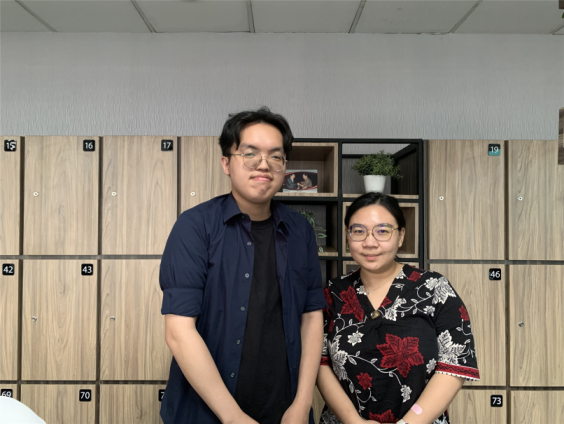
\includegraphics[width=7cm]{Gambar/bab2/dokumentasi-wawancara.jpg}
	\caption{Wawancara bersama \textit{Manager Human Resources} MyPassword}
	\label{fig:wawancara-manager-human-resources}
\end{figure}
\FloatBarrier

\subsection{Teori Umum}
\subsubsection{UML}
UML (\textit{Unified Modeling Language}) adalah bahasa grafis untuk menentukan, memvisualisasikan, membangun, dan mendokumentasikan artefak dari sistem perangkat lunak. Alat ini membantu dalam pemahaman yang lebih baik tentang perangkat lunak atau sistem atau produk yang akan dikembangkan, baik di antara pengembang maupun pelanggan~\cite{uml2022suriya}. Menurut Unhelkar~\cite{unhelkar2017software}, UML juga dapat membantu memodelkan persyaratan sistem baru dan membantu memahami proses bisnis dan aplikasi yang ada. Unhelkar juga menjelaskan terdapat beberapa jenis-jenis diagram UML:
\begin{enumerate}
    \item \textit{Use Case Diagram}
    \\ Memberikan gambaran umum tentang fungsionalitas sistem atau proses bisnis dari perspektif pengguna. Cara pengguna “menggunakan” sistem adalah titik awal untuk membuat diagram \textit{use case}.

    \item \textit{Activity Diagram}
    \\ Memodelkan aliran aktivitas normal dalam sistem dan alternatif serta pengecualian yang sangat baik digambarkan oleh diagram ini di mana saja interaksi terjadi. Khususnya, aliran dalam model \textit{use case} ke \textit{use case} di bawah diagram.

    \item \textit{Class Diagram}
    \\ Mewakili kelas, definisi mereka, hubungan, kelas dan entitas dari ruang masalah adalah entitas teknis terperinci di ruang solusi. Atribut dan operasi yang mendefinisikan kelas termasuk dalam diagram kelas ini. Hubungan dalam diagram kelas menggambarkan bagaimana kelas berinteraksi, berkolaborasi, dan mewarisi dari kelas lain.

    \item \textit{Sequence Diagram}
    \\ Memodelkan interaksi antar objek berdasarkan garis waktu mereka. Objek dapat berupa tabel, antarmuka pengguna, dan pengendali atau kelas lain juga dapat mewakili relasional untuk secara khusus ditunjukkan pada diagram ini atau mereka dapat menjadi objek anonim yang termasuk dalam suatu kelas. Urutan eksekusi pesan antar objek pada waktu runtime dimodelkan dengan baik oleh diagram ini, oleh karena itu namanya.
\end{enumerate}

\subsection{Gambar Diagram Rancangan Proses}
\subsubsection{\textit{Use Case Diagram}}
Pada rancangan \textit{use case diagram} untuk aplikasi presensi terdiri dari 3 aktor yaitu: (i) \textit{staff Infrastructure} dapat melakukan presensi masuk dan presensi keluar, serta melakukan pengajuan lembur, (ii) \textit{Manager Infrastructure} memiliki tugas untuk melakukan \textit{reject} atau \textit{penolakkan} pada data lembur yang tidak \textit{valid} dan melihat laporan lembur dan presensi (iii) \textit{Manager Human Resources} yang bertugas mengelola akun \textit{user}, melihat laporan data presensi dan lembur. \textit{Use case diagram} dari perancangan aplikasi presensi \textit{online} berbasis \textit{web} pada PT Password Solusi Sistem dapat dilihat pada \hyperref[sec:use-case-diagram-aplikasi-presensi-online]{\textbf{Lampiran~III}}.

Pada aplikasi presensi \textit{online}, \textit{staff Infrastructure} dapat melakukan \textit{login} dan \textit{logout} pada sistem, jika tidak memiliki akun dapat melakukan registrasi. \textit{Staff Infrastructure} dapat melihat jadwal jam kerja dan melakukan presensi masuk atau keluar, setelah itu mengaktifkan akses kamera dan lokasi, jika \textit{staff Infrastructure} melakukan presensi diluar jam \textit{shift} atau libur perusahaan maka sistem akan mengecek berdasarkan data \textit{shift} jam kerja \textit{staff Infrastructure} dan data hari libur perusahaan, jika syarat terpenuhi maka akan mencatat jam lembur tersebut. \textit{Staff Infrastructure} dapat melihat data riwayat presensi dan lembur, serta mengajukan \textit{form overtime request correction} jika \textit{staff Infrastructure} lupa melakukan presensi lembur. \textit{Manager Infrastructure} dan \textit{Manager Human Resource} memiliki beberapa akses yang sama seperti melakukan \textit{login} dan \textit{logout}, melihat data presensi dan lembur seluruh \textit{staff Infrastructure}, melakukan \textit{export} data presensi dan lembur dalam bentuk \textit{Microsoft Excel}, mengelola akun \textit{user} yang telah registrasi seperti mengaktifkan atau menonaktifkan, mengelola data hari libur perusahaan, mengelola \textit{shift} jam kerja \textit{staff Infrastructure} yang akan digunakan untuk pengecekkan presensi lembur. Selanjutnya perbedaan tambahan pada \textit{Manager Infrastructure} yaitu harus melakukan registrasi akun pada awal dan dapat melakukan penolakkan atau \textit{reject} pada data lembur \textit{Staff Infrastructure} yang tidak \textit{valid}.


\subsubsection{\textit{Use Case Scenario}}
\textit{Use case scenario} pada perancangan aplikasi presensi \textit{online} berbasis \textit{web} pada PT Password Solusi Sistem dapat dilihat pada \hyperref[sec:use-case-scenario-aplikasi-presensi-online]{\textbf{Lampiran~IV}}.

\subsubsection{\textit{Activity Diagram}}
\textit{Activity diagram} dari perancangan aplikasi presensi \textit{online} berbasis \textit{web} pada PT Password Solusi Sistem dapat dilihat pada \hyperref[sec:activity-diagram-aplikasi-presensi-online]{\textbf{Lampiran~V}}.

\subsubsection{\textit{Sequence Diagram}}
\textit{Sequence diagram} dari perancangan aplikasi presensi \textit{online} berbasis \textit{web} pada PT Password Solusi Sistem dapat dilihat pada \hyperref[sec:sequence-diagram-aplikasi-presensi-online]{\textbf{Lampiran~VI}}.

\subsubsection{\textit{Class Diagram}}
\textit{Class diagram} dari perancangan aplikasi presensi \textit{online} berbasis \textit{web} pada PT Password Solusi Sistem dapat dilihat pada \hyperref[sec:class-diagram-aplikasi-presensi-online]{\textbf{Lampiran~VII}}.